\section{Co-working aplikácie}
\indent Co-working aplikácie sú aplikácie, ktoré slúžia na komunikáciu a manažovanie tímu pri práci viac ľudí na dosiahnutie určitého cieľa alebo výsledku. Týchto aplikácii na trhu existuje veľa pričom niektoré sú bezplatné, niektoré sú platené a niektoré sú vyvinuté priamo vo firme kde sa používajú a nemá k nim teda prístup nikto okrem danej firmy. Medzi najznámejšie patrí napríklad Slack, Facebook workplace, Trello, Microsoft Teams a iné. 
\subsection{Slack}
\indent Slack je komunikačný nástroj vyvinutý pre pracovné využitie spoločnosťou Slack Technologies – „jedno miesto pre posielanie správ, nástroje a súbory“. To znamená, že Slack je softvér na posielanie „okamžitých“ správ s možnosťou pridania ďalších doplnkov podľa potreby používateľa. Tieto doplnky ale nie sú potrebné na plynulý chod aplikácie pretože základnou funkciou Slacku je len posielanie správ. Na Slacku existujú 2 spôsoby komunikácie: 1. spôsob sú tzv. kanály čo je v podstate skupinový rozhovor a 2. spôsob sú priame správy medzi dvoma ľuďmi. 
\subsubsection{História}
\indent Slack začal ako aplikácia na internú komunikáciu v spoločnosti Stewarda Butterfielda Tiny Speck pri vývoji online hry Glitch – hra bola vydaná v septembri 2011. Pre širšiu verejnosť bol Slack vydaný v auguste 2013. Slack je skratka pre: „Searchable Log of All Conversation and Knowledge“ čo vo voľnom preklade znamená „Protokol prehľadávania všetkých konverzácií a znalostí.“

\indent V marci 2015 spoločnosť Slack oznámila, že bola vo februári 2015 napadaná hackermi počas 4 dní. Počas tohto útoku boli ohrozené údaje používateľov. Medzi tieto údaje patrili e-mailové adresy, používateľské mená, heslá, telefónne čísla a Skype mená ktoré boli priradené k ich účtom. Po tomto útoku Slack pridal do svojej aplikácie dvojfaktorovú autentifikáciu. 
\subsubsection{Používateľské rozhranie}
\indent Keď chce používateľ začať používať Slack musí najskôr cez stránku Slacku vytvoriť názov svojej „inštancie“ Slacku. Tento názov sa potom stane súčasťou URL adresy, ktorá slúži ako pozvánka. Potom buď cez stránku Slacku alebo poslaním URL pozve ľudí, ktorých chce mať na svojom Slacku. 

\indent Po akceptovaní tejto pozvánky si používateľ vytvorí účet. Po prihlásení pod týmto účtom sa používateľovi otvorí stránka „inštancie“ Slacku alebo ak má nainštalovanú aplikáciu tak aplikácia Slacku viď. Obr.~\ref{fig:img-slack-app}

\indent Kanály na Slacku môžu byť verejné čo znamená, že každý člen skupiny ho vidí a môže sa k nemu pripojiť alebo súkromné čo znamená, že ich vidia len ľudia pridaný alebo pozvaný. Priame správy sú vždy súkromné ale môžu obsahovať až 8 ľudí.

\begin{figure}[H]
    \centering
    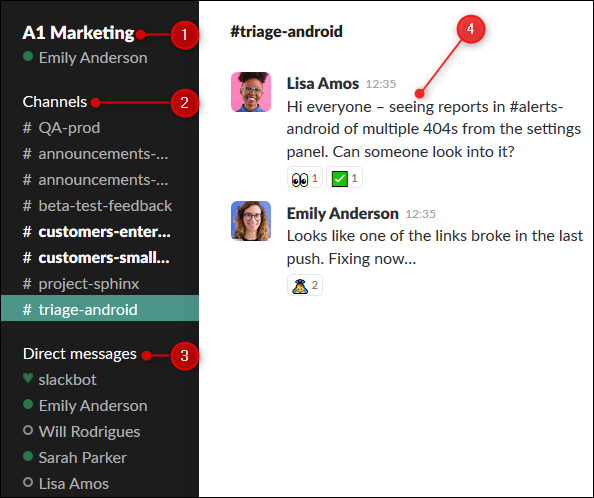
\includegraphics[scale=0.80]{img/obr1.png}
    \caption{Slack aplikácia}
    \label{fig:img-slack-app}
\end{figure}
\begin{enumerate}
    \centering
    \item Názov skupiny/inštancie
    \item Zoznam kanálov 
    \item Zoznam kontaktov
    \item Okno chatu
\end{enumerate}


\subsubsection{Doplnky}
\indent Do aplikácie Slack je možné pridať rôzne doplnky či už priamo vytvorené firmou Slack Technologies alebo inými firmami ako je Google, Jira, Trello a iné. Celkový prehľad doplnkov Slack uvádza na svojej stránke kde sa vie používateľ priamo prekliknúť aj na stránku daného doplnku kde je napísané čo doplnok prináša do Slacku plus tutoriál ako ho používať prípadne video používania doplnku. Doplnok je možné pridať priamo cez aplikácie Slack alebo cez stránku Slacku.

\indent Doplnky sú na stránke rozdelené do kategórii, do ktorých viac menej patria. Tieto kategórie sú rôzne od botov, ktorý automaticky ako je niečo zmenené na strane doplnkovej aplikácie, pridajú do daného kanála upozornenie alebo správu, až po priame importy, ktoré pridávajú funkcionalitu priamo do Slacku.
\subsubsection{Výber najznámejších importov}
\begin{itemize}
    \item Google Drive
    \item Google kalendár
    \item Trello
    \item Twitter
    \item Outlook kalendár
    \item OneDrive
    \item GitHub
    \item Polly(hlasovania a prieskumy)
    \item Jira Cloud
    \item TimeBot
    \item WorkBot
    \item Giphy
    \item Doodle Bot
\end{itemize}
\subsubsection{Cena}
\indent Slack ako taký je zadarmo ale sú tam isté obmedzenia. Hlavným obmedzením je prístup len k 10000 najnovším správam a používateľ môže pridať len 10 doplnkov na inštanciu. Ďalšími obmedzeniami sú napríklad žiadny jedno-kanálový alebo viac-kanálový hostia a limitované možnosti administrácie. 

\indent Ak chce používateľ sprístupniť celú funkcionalitu je to dosť drahé. Vychádza to približne 12 dolárov na používateľa mesačne pri ročnej platbe alebo približne 15 pri mesačnej platbe. Ak teda napríklad máme 1000 člennú skupinu, ktorá chce používať Slack vychádza to približne 144000 dolárov pri ročnej platbe.

\subsection{Facebook Workplace}
\indent Čas, ktorý ľudia strávili v práci chatovaním, prezeraním a likovaním príspevkov na Facebooku znižoval produktivitu ľudí cca v hodnote 3,5 bilióna dolárov. Táto téma sa pretriasala cez seriózne diskusie až po vytváranie vtipných obrázkov. Preto sa ľudia vo Facebooku začali zaoberať touto otázkou či sa funkcionalita Facebooku nedá preniesť aj na pracovnú aplikáciu. Toto dalo počiatok Facebook Workplacu, ktorý podľa slov jeho stvoriteľov má podporiť kolaboráciu tým, že ju urobí zábavnou a jednoduchšou pre ľudí.

\begin{figure}[H]
    \centering
    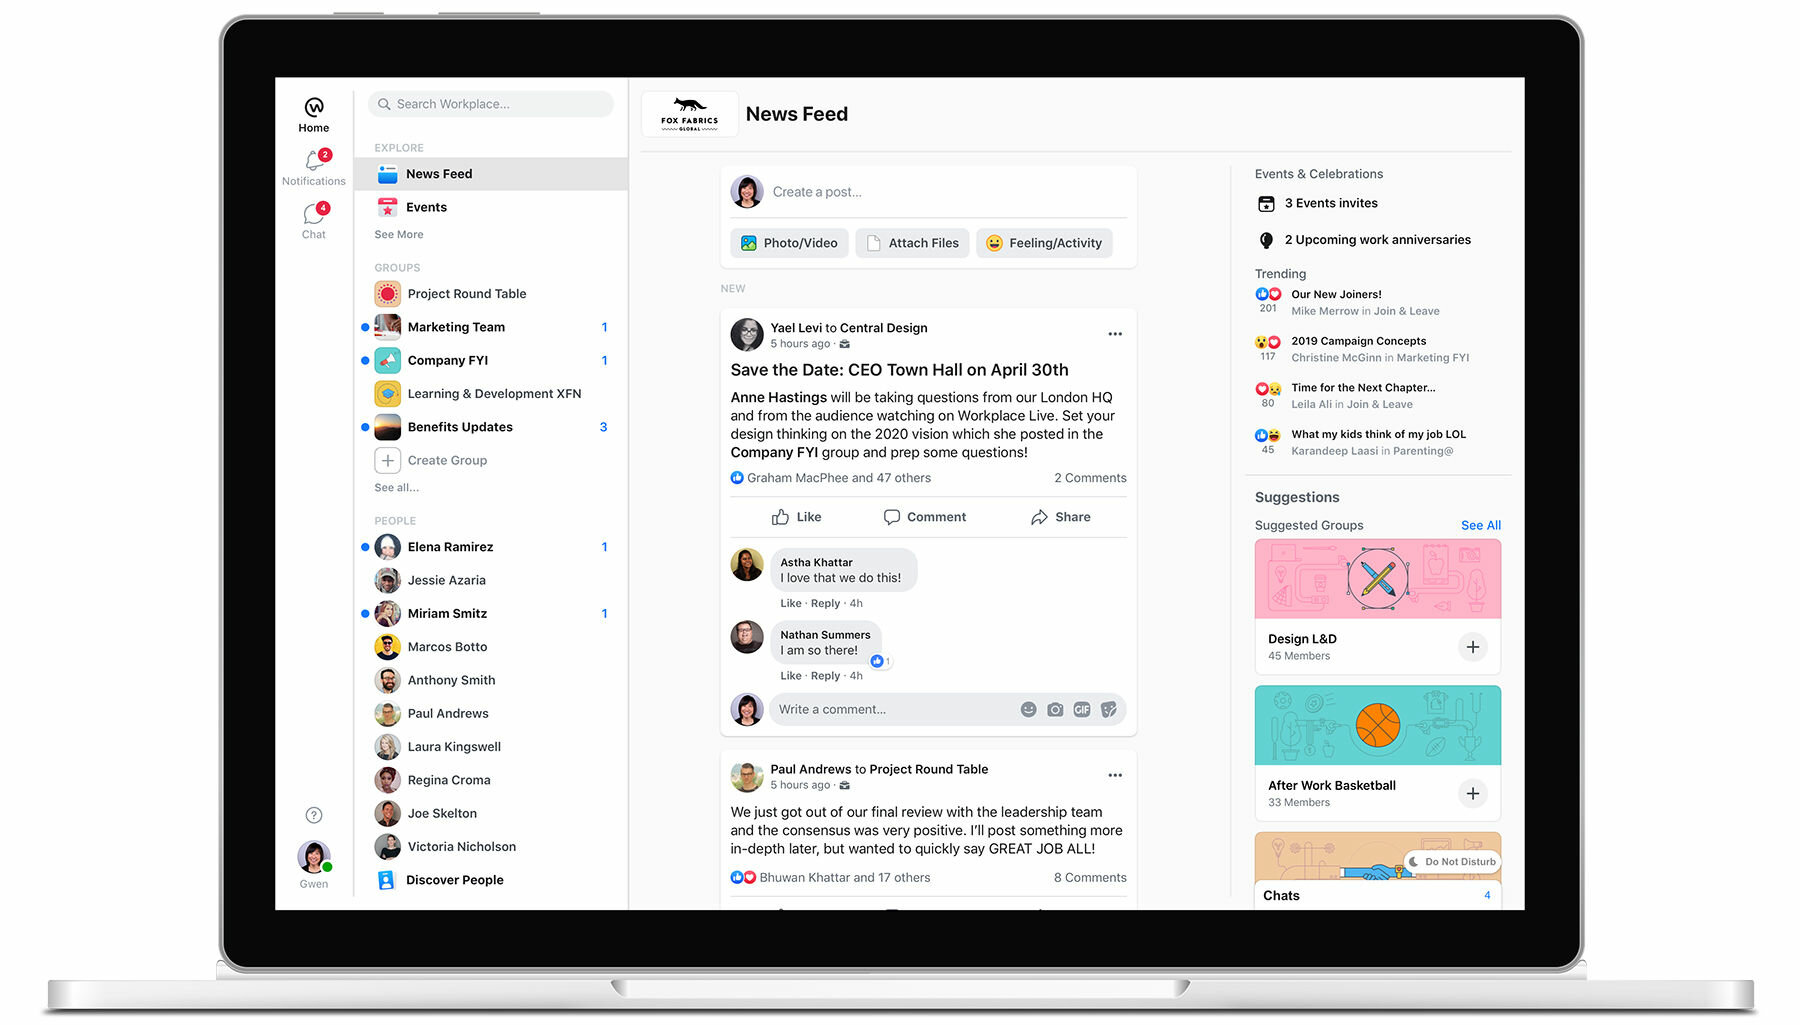
\includegraphics[scale=0.25]{img/obr-fb-workplace.jpg}
    \caption{Stránka Facebook Workplace}
    \label{fig:img-fb-workplace}
\end{figure}

\subsubsection{História}
\indent Myšlienka sa začala rozvíjať v roku 2014 keď prišla myšlienka nasmerovať tendenciu členov tímu prechádzať Facebook počas pracovnej doby k lepšej produktivite a spolupráci. Začiatkom roku 2015 sa začala do vybraných spoločností zavádzať beta verzia s názvom Facebook at Work. Keďže Facebook týmto vstupoval do neznámych vôd bolo samozrejmé, že beta verzia sa veľmi často menila. V polovici roka 2015 Facebook získal veľmi silného spojenca pre vývoj tejto aplikácie - The Royal Bank of Scotland – Škótska národná banka. Tá u seba presadila masívne využitie tejto beta verzie Facebook at Work kedy sa vytvorilo až 100000 nových účtov. 

\indent Ku koncu roka 2015 mal Facebook veľa kladných ohlasov na túto svoju vyvíjanú platformu od manažérov firiem kde bol Facebook at Work zavedený. Bolo to hlavne zapríčinené tím, že zamestnanci mali veľmi jednoduchý prístup k pracovným profilom svojich kolegov a podriadených. Tak isto kvôli prehľadnosti sa názov zmenil na Facebook Workplace.

\indent  V októbri 2016 boli oficiálne na trh uvedené pracovné a mobilné verzie aplikácie Facebook Workplace. Týmto Facebook začal konkurovať gigantom ako Slack a Microsoft Teams (vtedy Skype for Business) na poli podnikového softvéru.
\subsubsection{Používateľské rozhranie}
\indent Rozhranie Workplacu je podľa slov používateľov na 95\% rovnaké ako to na Facebooku. Väčšina populárnych funkcii Facebooku bola pridaná tiež do Workplacu:
\begin{itemize}
    \item Newsfeed – zobrazujú sa tu všetky tímové aktivity ako napríklad príspevky členov tímu, firemné akcie a všetky informácie týkajúce sa práce prihláseného používateľa
    \item Live tools – funkcie na živý prenos (Live streaming)
    \item Skupiny – manažéri môžu vytvárať skupiny na pracovisku a tým udržiavať aktivity jednotlivých skupín/tímov na jednom  mieste
    \item Správy – používatelia si môžu písať so svojimi kolegami
\end{itemize}

\indent Pre používateľov je toto síce výhoda keďže sa nemuseli učiť používať nový nástroj avšak pre firmy je problém prijať v podstate napodobeninu Facebooku ako pracovnú aplikáciu. Kvôli tomuto Facebook aj oddelil profily Facebooku a Workplacu nakoľko do nedávna boli tieto profily prepojené a aj vytváranie účtu sa robilo cez profil Facebooku. 
\subsubsection{Cena}
\indent Workplace je pre firmy na prvé tri mesiace zadarmo. Potom sa jeho cena odvíja od počtu aktívnych účtov. Do 1000 používateľov sa platia 3 doláre za každého, do 10000 používateľov sa platí 2 doláre za každého a nad 10000 používateľov sa platí 1 dolár za každého.  Pre neziskové organizácie a akademické účely je úplne zadarmo aj po 3 mesiacoch.

\subsection{Microsoft Teams}
\indent Microsoft Teams je aplikácia na pracovnú komunikáciu a kolaboráciu od spoločnosti Microsoft, ktorá bola vyvinutá aby konkurovala aplikáciám Slack, Workplace, HipChat. Vo svojej najjednoduchšej podobe je to aplikácia umožňujúca komunikáciu medzi členmi vytvorenej skupiny na báze miestností - kanálov. Microsoft sa už pred vydaním Teams pokúšal presadiť na trhu pracovných aplikáciu pomocou svojho Skype for Business. Táto aplikácia avšak nenaplnila očakávania tak ako jej lepšia verzia Teams. 
\subsubsection{História}
\indent V marci 2016 chcel Microsoft kúpiť Slack za 8 miliárd dolárov avšak Bill Gates bol proti a skôr presadzoval zlepšenie ich aplikácie Skype for Business. Tento nákup presadzoval hlavne vysoko postavený pracovník Microsoftu Qi Lu. Ten avšak ešte v roku 2016 opustil spoločnosť a v Novembri toho istého roku Microsoft oznámil prácu na aplikácii Teams ako na aplikácii, ktorá má konkurovať Slacku. 

\indent Slack uznal Teams ako konkurenčnú službu avšak uviedol, že nekonkurujú rovnakému publiku nakoľko Teams v tej dobe neumožňoval ľudom bez predplateného balíka Office 365 vstup do aplikácie Teams. Slack to zdôvodňoval aj tým, že neprepokladá sa, že by malé a stredné podniky, ktoré už Slack používajú nezačnú používať platenú službu Office, ktorej Teams bol súčasťou. Neskôr však Teams pridal možnosť pridania nových ľudí aj bez predplateného balíka Office 365. Slack na toto reagoval integráciou služieb od Google (Drive, Kalendár, Gmail). 

\indent V roku 2017 sa udiali 2 udalosti. Prvou bolo, že Teams nahradili MS Classroom v balíku Office 365 for Education. Druhou udalosťou bola správa v septembri, že Teams nahradzujú Skype for Business. Tým bola aj ukončená služba Skype for Business. 

\begin{figure}[H]
    \centering
    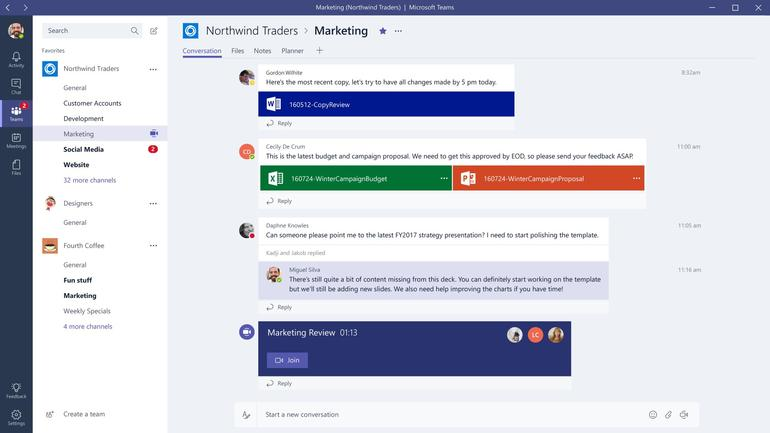
\includegraphics[scale=0.70]{img/obr-ms-teams.jpg}
    \caption{Aplikácia MS Teams}
    \label{fig:img-ms-teams}
\end{figure}

\indent V júli 2018 oznámil Microsoft bezplatnú verziu služby Teams s obmedzeniami typu počet používateľov a kapacitu ukladania súborov. V novembri 2019 dosiahol Teams 20 miliónov používateľov čo bol nárast o 7 miliónov od júla 2019. 
\subsubsection{Používateľské rozhranie}
\indent Rozhranie Teams je veľmi podobné tomu na Slacku. Na vytvorenie tímu treba vytvoriť URL, ktorá potom slúži rovnako ako na Slacku na pozívanie používateľov. Po prihlásení sa pomocou Microsoft účtu potom môžu už jednotlivý používatelia vytvárať miestnosti, do ktorých môžu pridávať príspevky. Tak isto je možná komunikácia medzi používateľmi bez miestnosti štýlom ako je v aplikácii Skype. Tu je povolená aj hlasová a video komunikácia Skype štýlom. 

\indent Mimo klasických miestností-kanálov je možne vytváranie aj takzvaných meeting miestností, ktoré slúžia na komunikáciu počas pracovných porád, meetingov a stretnutí. Tieto miestnosti umožňujú priame pridanie času a dátumu meetingu do kalendára Outlooku Náhľad nástenkya po otvorení miestnosti je možné vidieť v akom stave stretnutie je: ešte nezačalo, prebieha, ukončené. 

\indent Microsoft do Teams pridal aj funkciu podobnú funkcionalite Trella – dashboard. Pomocou tejto funkcie môžu manažéri, učitelia, vedúci prideľovať a sledovať prácu používateľov. Tak isto sa jednotlivé úlohy na tejto „nástenke úloh“ dajú komentovať, presúvať alebo hodnotiť.

\indent Samozrejmosťou je veľmi dobrá kompatibilita s inými aplikáciami Microsoftu ako je Word, Excel, PowerPoint, OneDrive. Jednotlivé dokumenty týchto aplikácii sa dajú priamo posielať, upravovať v aplikácii Teams a tak majú jednotlivý používatelia vždy najaktuálnejšiu verziu dokumentu k dispozícii. Microsoft pridal ale aj komunikáciu s aplikáciami od iných vývojárov ako je GitHub, Evernote, Zendesk pomocou konektorov. Táto komunikácia slúži najmä na posielanie upozornení, že na strane druhej aplikácii prišlo k nejakej zmene – napríklad príde upozornenie do miestnosti, že niektorý používateľ pushol na git niečo nové.  
\subsubsection{Doplnky}
\indent Do Teams podobne ako do Slacku je možne pridanie rôznych doplnkov od iných vývojárov. Tieto doplnky sú avšak po väčšine len Boti, ktorých úlohou je posielanie upozornení, že na strane druhej aplikácie prišlo k nejakej zmene – pridanie nových vecí na github, zmena v Evernote a iné. Týchto Botov je potvrdených zatiaľ 85 a 70 konektorov – aplikácie, ktoré slúžia nielen na posielanie upozornení. 
\subsubsection{Cena}
\indent Microsoft Teams je v svojej jednoduchšej podobe zadarmo. Obmedzeniami bezplatnej verzie sú napríklad prístup na OneDrive, plánovania schôdze, nahrávanie schôdze pomocou Microsoft Stream, technická podpora, viacfaktorová autentifikácia pre všetkých používateľov. 

\indent Platených verzii je viac. Tieto verzie sú viazané na balík Office 365, ktorý má používateľ/firma zaplatený. Za balík Office 365 Business Essentials pýta Microsoft 4,20€ za používateľa mesačne s ročnou viazanosťou a za balík Office 365 Business Premium 10,50€ za používateľa mesačne tak isto s viazanosťou na rok. V balíku Premium je zahrnutá všetka funkcionalita aplikácie Teams. Pri balíčku Essentials sú tam stále isté obmedzenia.

\subsection{Trello}
\indent Trello je aplikácia na vytváranie pracovnej nástenky v kanbanskom štýle. Aplikácia od roku 2017 patrí spoločnosti Atlassian avšak vydaná bola v roku 2011 spoločnosťou Fog Creek Sowtvare. Aplikácia obsahuje virtuálnu nástenku kde členovia tímu môžu vytvárať, organizovať a priraďovať úlohy v rámci projektu. Použitý kanbanský/kartový štýl umožňuje členom tímu vzájomne spolupracovať a komunikovať pri práci na projekte. Používatelia môžu k projektovým kartám pridávať komentáre, odkazy, súbory a fotografie. Trello existuje v rôznych podobách. Existuje webová aplikácia, desktopová aplikácia či už pre Windows alebo MacOS a tak isto existujú aj mobilné aplikácie pre Android a iOS. Existuje aj import aplikácie do Slacku.
\subsubsection{Kanbanská nástenka}
\indent Kanbasnká nástenka je agilný nástroj na riadenie projektov navrhnutý tak, aby pomohol vizualizovať priebeh projektu a maximalizovať efektívnosť. Na kanbanskej nástenke sa používajú karty, stĺpce a neustále zlepšovanie. Toto má za následok jednoduchú vizualizáciu prebiehajúcej práce a tým vedúcim tímov pomáhať lepšie manažovať prácu tímu. 

\begin{figure}[H]
    \centering
    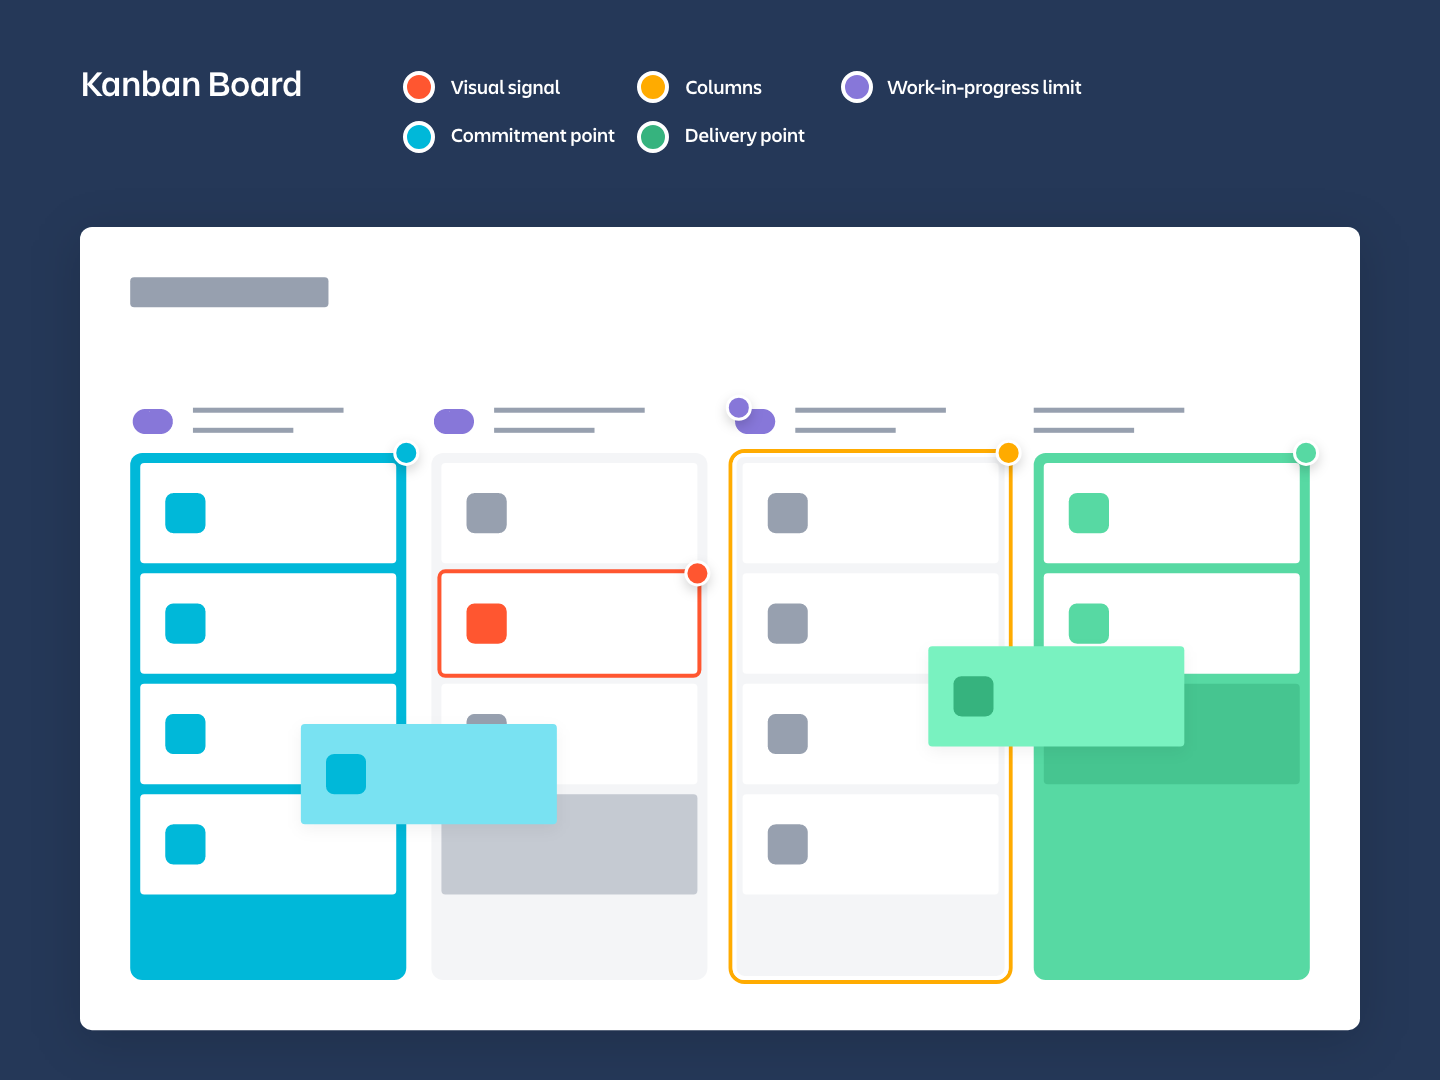
\includegraphics[scale=0.30]{img/obr4.png}
    \caption{Jednoduchá kanbasnká nástenka}
    \label{fig:kab-nas}
\end{figure}

\subsubsection{História}
\indent Trello bolo spustené v roku 2011 spoločnosťou Fog Creek. Za celou myšlienkou bol hlavne zakladateľ spoločnosti Joel Spolsky. Magazín Wired zaradil aplikáciu do „The 7 Coolest Startups You Haven´t Heard of Yet“ – Najlepších 7 startupov, o ktorých ste nepočuli. Tak isto sa v článku objavil názor, že Trello uľahčuje a svojim spôsobom spríjemňuje prácu na projektoch. 

\indent V máji 2016 ohlásilo Trello, že dosiahlo 1,1 milióna aktívnych používateľov denne a 14 miliónov celkovo založených účtov. V januári 2017 spoločnosť Atlassian kúpila Trello za 425 miliónov dolárov s tým, že 22\% podielu stále ostávala v rukách investorov a zakladateľa Joela Spolskeho. V roku 2019 nastal rapídny nárast používateľov kedy ešte v marci malo Trello 35 miliónov používateľov ale už v októbri to bolo 50 miliónov.
\subsubsection{Používateľské rozhranie}
\indent Prostredie aplikácie je veľmi jednoduché na používanie a nemá v sebe veľa zbytočných vecí. Tak isto navigácia v prostredí je veľmi jednoduchá a intuitívna. Registrácia je veľmi jednoduchá. Jediné čo nový používateľ potrebuje je meno, heslo a email. 

\indent Hneď po prihlásení sa používateľovi zobrazí nástenka kde vidí tímy, v ktorých je pridaný. Tak isto môže vytvoriť novú kartu tímu. Po vytvorení sa otvorí okno tímu, ktoré zväčša pozostáva z 3 stĺpcov – To Do, Doing a Done plus možnosť pridať ďalšie stĺpce. Tri dopredu vytvorené stĺpce sa samozrejme dajú vymazať alebo premenovať. 

\begin{figure}[H]
    \centering
    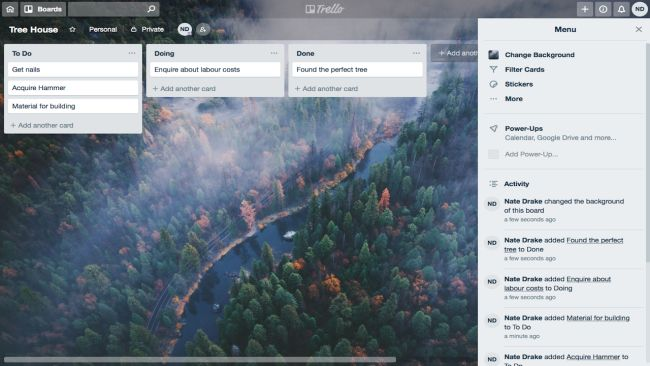
\includegraphics[scale=0.65]{img/obr-trello.jpg}
    \caption{Náhľad nástenky}
    \label{fig:nastenka}
\end{figure}

\indent V jednotlivých stĺpcoch je potom možné vytvárať nové karty, ktoré reprezentujú nejakú úlohu, komunikáciu alebo čokoľvek čo tím potrebuje. Po kliknutí na kartu sa zobrazí okno kde sa nachádza popis karty, komentáre a možnosti čo sa dá s kartou robiť – priradiť kartu používateľom aby pri zmene na karte dostali upozornenie. Upozornenia sa dajú samozrejme aj vypnúť. Na jednotlivé nástenky je možné pridanie rôznych doplnkov ako je napríklad kalendár, Googke drive, Slack, Mapy alebo špecifické doplnky. 

\indent Po kliknutí na profil sa otvorí stránka používateľského profilu. Tu je možne zmeniť meno, pridať fotku profilu, zmeniť iniciály, zmeniť avatara z iniciálok na fotku, nastaviť politiku upozornení alebo pre farebne slepých používateľov je tu možnosť zapnutia módu pre farebne slepých. 

\begin{figure}[H]
    \centering
    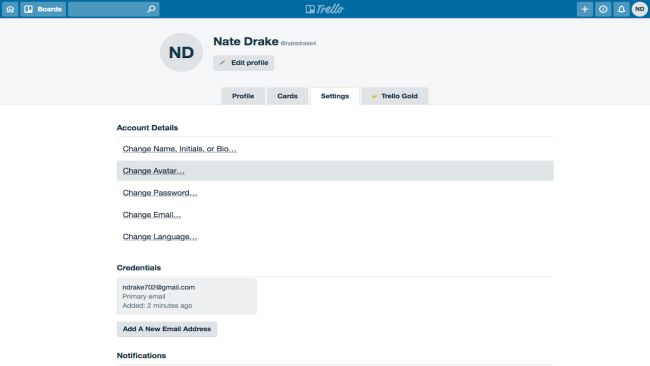
\includegraphics[scale=0.65]{img/obr-trello-profil.jpg}
    \caption{Stránka profilu}
    \label{fig:profil}
\end{figure}

\subsubsection{Doplnky}
\indent Do jednotlivých násteniek alebo tímov sa dajú pridať rôzne doplnky, ktoré rozširujú možnosti použitia Trella. Okrem rôznych Botov, ktorí len posielajú preddefinované správy alebo upozornenia je ponuka doplnkov veľmi veľká – od štandardných doplnkov ako je kalendár, Dropbox, Google Drive, Slack, GitHub, až po špecifické určené nie len na co-working ako napríklad Card Family, Prize Checker, Prize Tag a iné. 
\subsubsection{Cena}
\indent Trello ponúka 3 typy účtov. Bezplatný, ktorý zahŕňa neobmedzený počet násteniek, kariet, členov tímu alebo príloh. Je možne pridať jeden doplnok na nástenku a je možné pridanie prílohy o veľkosti do 10MB alebo prepojiť akýkoľvek súbor z Google Drive, Dropbox alebo OneDrive účtu. 

\indent Business balík stojí 9,99\$ mesačne ale platí sa ročné predplatné. Balík ponúka to isté čo bezplatný balík s tým, že je možne pridať neobmedzený počet doplnkov na nástenku a je možné pridať 250MB prílohy. Ďalšími rozširujúcimi vecami je možnosť usporiadania násteniek do kolekcii, nastaviť kto tieto kolekcie môže vidieť alebo nahratie vlastných pozadí pre nástenky. 

\indent Enterprise balík stojí 20,83\$ mesačne pri ročnom predplatnom. Balík zahŕňa funkcionalitu Business balíka plus dvojfaktorová autentifikácia, šifrovanie súborov, vlastná kontrola zabezpečenia, vylepšené SLA. 

\section{Návrh a implementácia aplikácie}
\indent Témou diplomovej práce je implemetovať co-working aplikáciu s využitím webového frameworku Ionic/Angular s neskorším exportom na desktopovú aplikáciu pomocou Electronu na strane frontendu a s použitím Node.js a CouchDB na strane servera. V tejto kapitole sa budeme zaoberať návrhom celej aplikácie s využitím daných technológii na jednotlivých komponentoch. 

\begin{figure}[H]
    \centering
    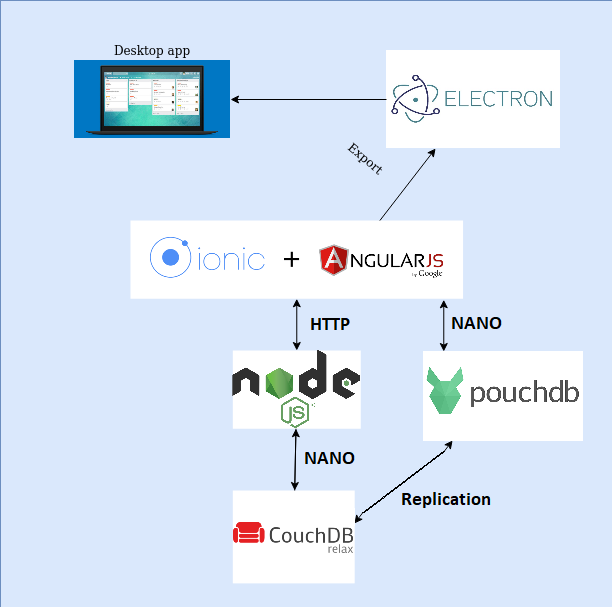
\includegraphics[scale=0.60]{img/diagram.png}
    \caption{Návrh komunikácie medzi komponentami}
    \label{fig:diagram}
\end{figure}

\indent Po prieskume aktuálnych technológii sme sa rozhodli využiť Node.js ako náš server, ktorý bude komunikovať s našou NoSql databázou CouchDB, do ktorej bude ukladať zadané dáta a zároveň posielať žiadané dáta na frontend implementovaný pomocou typescriptovo založeného frameworku Ionic. Ionic sa avšak ako bolo spomenuté v kapitole .... využíva na tvorbu webových alebo mobilných aplikácii. Preto finálnu webovú aplikáciu exportujeme nakoniec pomocou Electronu na desktopovú aplikáciu pre platformu Windows/Linux/MacOS.

\subsection{Špecifikácia požiadaviek}
\indent Prvým krokom pri tvorbe návrhu je špecifikovanie vlastností a celkového správania aplikácie. Definuje sa tu funkcionalita, ktorú chceme aby naša aplikácia mala, správanie aplikácie v určitých situáciách a jej kľúčové parametre, ktoré musí podľa požiadaviek spĺňať.
\subsubsection{Používateľské požiadavky} 
\indent Používateľské požiadavky sa stanovili na základe prehľadu co-working aplikácii, ktoré už existujú. Za základ sa zobrali hlavné funkcionality Slacku a k nim sa pridali buď doplnky Slacku alebo funkcie iných aplikácii. Softvér bude mať 2 používateľské rozhrania kedy jedno bude slúžiť ako administrátorské určené pre vedúcich tímov a klasické prostredie určené pre členov tímu. Administrátorské konto bude mať možnosť sa medzi týmito dvoma prostrediami prepínať. Administrátorské prostredie bude umožňovať vytváranie tímov, pozívanie a pridávanie členov tímu a manažovanie taskov. Používateľské prostredie bude umožňovať vytváranie miestností na stránke tímu, vytváranie stretnutí, zahajovanie hlasovaní, pridávanie príspevkov do miestností, komentovanie príspevkov, komunikáciu medzi členmi tímu, pridanie kontaktu, akceptovanie alebo zamietnutie pozvánky do tímu, správu svojich taskov.

\textbf{Funkcionálne požiadavky:}

\underline{\textit{Administrátor:}}
\indent\begin{itemize}
    \item Prihlásenie a odhlásenie
    \item Vytvorenie tímu
    \item Pridanie používateľa do tímu
    \item Vytvorenie tasku
    \item Pridanie používateľa do tasku
    \item Nastavenie stavu tasku
    \item Prepnutie sa medzi rozhraniami aministrátor a používateľ
\end{itemize}


\underline{\textit{Používateľ:}}
\indent\begin{itemize}
    \item Prihlásenie a odhlásenie
    \item Akceptovanie pozvánky do tímu
    \item Pridanie miestnosti v tíme a nastavenie či bude verejná alebo súkromná
    \item Pridanie ľudí do miestnosti ak je súkromná
    \item Pridanie udalosti v tíme
    \item Spravovanie svojich taskov
    \item Zahájenie hlasovania
    \item Pridanie kontaktu do svojho zoznamu kontaktov
    \item Nápisanie správy inému používateľovi
    \item komentovanie príspevkov v miestnosti
    \item Prezeranie svojho kalendára\newline
\end{itemize}


\textbf{Nefunkcionálne požiadavky:}
\indent\begin{itemize}
    \item Používateľsky prijateľné prostredie
    \item Obsluha viacerých používateľov
    \item Používateľské rozhranie implementované prostredníctvom desktopovej aplikácie
    \item Dizajn inšpirovaný aplikáciou Slack
\end{itemize}